\documentclass[12pt, letterpaper]{ctexrep}

\usepackage{titling}
\usepackage{standalone}
\usepackage{fontenc}


\usepackage[x11names]{xcolor}
\definecolor{SaddleBrown}{rgb}{0.55, 0.27, 0.07}
\definecolor{IndianRed}{rgb}{0.80, 0.36, 0.36}
\definecolor{Firebrick}{rgb}{0.70, 0.13, 0.13}
\definecolor{DarkBlue}{rgb}{0, 0, 0.55}
\definecolor{Goldenrod}{rgb}{0.85, 0.65, 0.13}
\definecolor{Peru}{rgb}{0.85, 0.65, 0.13}




\usepackage{hyperref}
\hypersetup{
    colorlinks=true,
    linkcolor=DarkBlue,
    urlcolor=blue,
    linktoc=all
}
\setcounter{tocdepth}{1}


\usepackage{mathtools}
\usepackage{amsmath}
\usepackage{tikz}
\usepackage{verbatim}
\usetikzlibrary{calc}

% put color to \boxed math command
\newcommand*{\boxcolor}{Peru}
\makeatletter
\renewcommand{\boxed}[1]{\textcolor{\boxcolor}{%
\tikz[baseline={([yshift=-1ex]current bounding box.center)}] \node [rectangle, minimum width=1ex,rounded corners,draw] {\normalcolor\m@th$\displaystyle#1$};}}
\makeatother


\usepackage{listings}

\definecolor{codegreen}{rgb}{0,0.6,0}
\definecolor{codegray}{rgb}{0.5,0.5,0.5}
\definecolor{codepurple}{rgb}{0.58,0,0.82}
\definecolor{backcolour}{rgb}{0.95,0.95,0.92}

\lstdefinestyle{mystyle}{
    backgroundcolor=\color{backcolour},
    commentstyle=\color{codegreen},
    keywordstyle=\color{magenta},
    numberstyle=\tiny\color{codegray},
    stringstyle=\color{codepurple},
    basicstyle=\ttfamily\footnotesize,
    breakatwhitespace=false,
    breaklines=true,
    captionpos=b,
    keepspaces=true,
    numbers=left,
    numbersep=5pt,
    showspaces=false,
    showstringspaces=false,
    showtabs=false,
    tabsize=2
}

\lstset{style=mystyle}


\usetikzlibrary{positioning}
\usetikzlibrary{petri} % LATEX and plain TEX
\usetikzlibrary[petri] % ConTEXt
\usepackage{pgfplots}
\pgfplotsset{compat=1.13}


\usepackage{framed}
\usepackage{quoting}

\colorlet{shadecolor}{LightSteelBlue1}
\usepackage{lipsum}
\newenvironment{shadedquotation}
 {\begin{shaded*}
  \quoting[leftmargin=5pt, rightmargin=5pt, vskip=0pt]
 }
 {\endquoting
 \end{shaded*}
}


\usepackage{lipsum} % for dummy text
\usepackage{enumitem}
\setlist{nosep} % or \setlist{noitemsep} to leave space around whole list

\pagestyle{plain}

\usepackage{ctex}
\usepackage{xeCJK}
\xeCJKsetup{CJKmath=true}


\usepackage[
    left=1.0in,
    right=1.0in,
    top=1.5in,
    bottom=1.5in,
]{geometry}


\setlength{\droptitle}{-18em}
\title{\fontsize{40}{20} \textbf{\textcolor{red}{\kaishu 趣题集}}}
\author{\textcolor{red}{南方小智}}
\date{\textcolor{red}{\today}}

\usepackage{eso-pic}
\newcommand\BackgroundPic{%
\put(0,0){%
\parbox[b][\paperheight]{\paperwidth}{%
\vfill
\centering
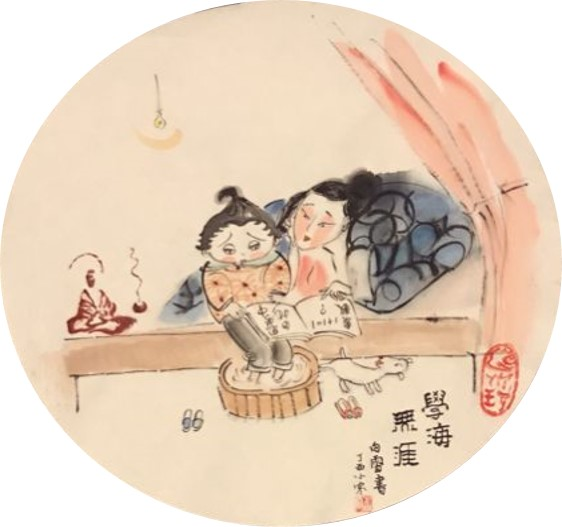
\includegraphics[width=\paperwidth,height=\paperheight,%
keepaspectratio]{images/趣题集/background.jpeg}%
\vfill
}}}



\begin{document}
\AddToShipoutPicture*{\BackgroundPic}
\maketitle
\thispagestyle{empty}
\newpage

\setcounter{page}{1}
\tableofcontents
\newpage

本书共分为十章,每章分为十节,每节都会讨论一个趣题,总共100个趣题。更多的趣题会编入到下一部趣题集中。

\chapter{概率}


本章讨论和概率统计有关的话题。
\subsection{测试}
测试MAIN文件中的标题。

\section{苏格拉底的麦穗}
\begin{shadedquotation}
\noindent
苏格拉底和弟子们走到一片麦田里,风吹麦浪,阵阵秋意袭来。苏格拉底对弟子们说,“你们从麦田的这一头走到那一头,中间可以拾起一株麦穗,我们看看谁能找到最大的麦穗。” 他接着说 “当然,你们只有一次机会,一旦选定了,之后即便遇到更大的麦穗,也不能再采摘;而且你们也不能回头去采摘那些已经错过的大麦穗。” 弟子们听完之后,面面相觑。
\end{shadedquotation}


为了拿到最大的麦穗,你会采取什么样的策略呢?当然,按照既定的策略,我们也许不能保证拿到最大的麦穗,但是我们可以使得拿到最大麦穗的概率最大化。也就是说,拿到最大麦穗的概率就是我们的收益。

假设麦田里有n株麦穗,如果我们的策略是随机地选择一株麦穗,那么,我们的收益将是1/n。

那么,有没有一种策略能够比随机选择更好一些呢?

事实上,我们可以对麦穗的大小分布先观察一段时间,通过我们观察到的麦穗分布,我们就有了一些信息为我们接下来的选择提供依据,从而提升拿到最大麦穗的概率。为了说明这种方法,我们考虑一个只有“三株麦穗”的情景。

\begin{shadedquotation}
\noindent
商场里举行抽奖活动,获奖的顾客可以选择在三件礼品里挑一件。刚开始,顾客并不知道这三件礼品是什么。然后,这三件礼品将被工作人员随机逐个展示出来,每件礼品展示出来后,顾客可以选择要这件礼品,也可以pass掉这件礼品。如果顾客选择pass,工作人员将展示下一件礼品,以此类推。那么,使用什么策略,可以让顾客更有可能挑选到价值最高的礼品呢?
\end{shadedquotation}


我们假设这三件礼品分别是\textbf{\textcolor{Firebrick}{手套}},\textbf{\textcolor{Firebrick}{电视}},还有\textbf{\textcolor{Firebrick}{车子}}。显然顾客是想要选到车子的,但是刚开始的时候,顾客并不知道这三件礼品是什么。

让我们来考虑一下以下这种策略:

\begin{enumerate}
\item{ 第一件礼品直接pass掉,仅仅把这件礼品的价值记下来; }
\item{ 第二件礼品如果比第一件礼品贵,则选第二件礼品; }
\item{ 否则,选第三件礼品。 }
\end{enumerate}


我们知道,三件礼品的出场顺序总共有六种,如果我们采取随机选择策略,我们将有1/3的概率抽到车子。但是,如果我们采取上面的策略,在不同的礼品出场顺序下,我们将得到如下结果:


\begin{itemize}
\item{ 手套 → 电视 → 车子:将会得到\textbf{\textcolor{Firebrick}{电视}} }
\item{ 手套 → 车子 → 电视:将会得到\textbf{\textcolor{Firebrick}{车子}} }
\item{ 电视 → 手套 → 车子:将会得到\textbf{\textcolor{Firebrick}{车子}} }
\item{ 电视 → 车子 → 手套:将会得到\textbf{\textcolor{Firebrick}{车子}} }
\item{ 车子 → 手套 → 电视:将会得到\textbf{\textcolor{Firebrick}{电视}} }
\item{ 车子 → 电视 → 手套:将会得到\textbf{\textcolor{Firebrick}{手套}} }
\end{itemize}


我们可以看到,有三种排列的情况下,也就是1/2的概率,我们能拿到车子,而只有1/6的概率,我们会拿到手套。这种策略的收益,显然要比随机选择策略要好。因为我们首先对礼品进行了观察,而我们接下来的策略也是基于我们观察到的信息的,所以我们得到更好的结果也就理所当然了。

如果我们把我们的这种策略推广到n件礼品,就变成了和苏格拉底的麦穗一样的问题。我们可以制定类似的策略:

\begin{enumerate}
\item{ 前r株麦穗直接pass掉,仅仅记下r株里面最大麦穗的大小,记作M; }
\item{ 接下来的麦穗如果比M要大,那就选这一株麦穗; }
\item{ 如果到最后更好的麦穗都没有出现,就选择最后一株麦穗。 }
\end{enumerate}


\subsection{如何选择r}

那么,我们应当如何选择首先观察多少麦穗呢?也就是如何确定r呢?如果我们观察了太多,那么我们很有可能会把最大的麦穗给pass掉。如果我们观察的麦穗太少,我们很可能最后会选到一株大小平庸的麦穗。下面我们来计算对于一个确定的r,我们能找到最大麦穗的概率:


$$\boxed{
\begin{aligned}
\text{P}(r) &  = \sum_{k=r+1}^n{
	\text{P}(
		第 k 个是最大的麦穗的并且被选中
	)
} \\\\
&  = \sum_{k=r+1}^n{
	\text{P}(
		第 k个是最大的麦穗
	)
	\text{P}(
		第k个被选中|第 k个是最大的麦穗
	)
} \\\\
&  = \sum_{k=r+1}^n{
	\frac{1}{n}
	\text{P}(
		前k-1个中的最大的麦穗出现在前r个里
	)
} \\\\
& = \sum_{k=r+1}^n{
	\frac{1}{n} \frac{r}{k-1}
} = \frac{r}{n} \sum_{k=r+1}^{n}{\frac{1}{k-1}}
= \frac{r}{n} \sum_{k=r}^{n-1}{\frac{1}{k}}
\end{aligned}
}$$

注意到如果想要选中第k个,要满足

\begin{enumerate}
\item{ k比前面的麦穗都要大,而当k是最大的麦穗时,这一点是显然满足的。 }
\item{ 前k-1株麦穗中最大的麦穗在前r株里,否则,这株较大的麦穗就会抢在k之前被选中。 }
\end{enumerate}


所以我们有上式中的推断:

$$\boxed{
\text{P}(
		第k个被选中|第 k个是最大的麦穗
) \\\\ =
\text{P}(
		前k-1个中的最大的麦穗出现在前r个里
	)
}$$

接下来我们来估算当r变化时,P(r)的最大值。我们考虑将P(r)的表达式近似地连续化,得到:

$$\boxed{
\newcommand{\ud}{\mathrm{d}}
\begin{aligned}
\text{P}(r) &  = \frac{r}{n} \sum_{k=r}^{n-1}{\frac{1}{k}}  \approx \frac{r}{n} \int_r^n\frac{1}{x} \ud x \\\\
& = \frac{r}{n} (\log(n) - \log(r)) = \frac{r}{n}\log(\frac{n}{r}) \\\\
& = -x\log(x), 其中x=\frac{r}{n}
\end{aligned}
}$$


通过求导我们可以知道x=1/e时,P(r)取得最大值1/e。其中e就是自然对数的底,e约等于2.71828。

\textbf{\textcolor{Firebrick}{因此,在麦田里,当麦穗很多的时候,我们应当首先观察前1/e$\approx$37\%的麦穗,然后在接下来的麦穗中选择一株比观察到的所有麦穗还要大的一株麦穗。}}这样,我们找到最大麦穗的概率就会接近1/e!当n很大的时候,1/e的收益和随机选择策略得到的1/n的收益相差甚远。

\subsection{结语}

现实生活中,以苏格拉底的麦穗为模型的场景有很多,这些场景都可以利用我们今天所讨论的策略。比如我们去买房子或者租房子,事先打算看十套房;我们打算和多个姑娘谈恋爱,而最终只和一个姑娘结婚;我们打算招聘一个会计师,而打算举行六场面试;在炒股的时候我们想低买高卖,如何能够更高概率找到这些最值点等等。

在数学中,苏格拉底的麦穗这个问题的模型是最优停止理论的一个特例。这类问题还有什么应用?是否存在比我们今天讨论的策略更优的策略?有兴趣的朋友可以阅读一下本文的参考文献:\href{http://www.math.ucla.edu/~tom/Stopping/Contents.html}{Optimal Stopping and Applications}

总之,看完苏格拉底的麦穗这个故事,我们明白了一个道理:\textbf{\textcolor{Firebrick}{千万不要和初恋结婚啊!}}


\section{男孩国}
\begin{shadedquotation}
\noindent
从前有一个国王,重男轻女的思想非常的严重,他颁布了一条法令,任何夫妻,如果第一胎生下了男孩,就不许再生了;如果第一胎生下的是女孩,就一定要继续生,直到生下一胎男孩为止。如果生男生女的概率是一样的,都是50\%,那么,在这条法令的作用下,王国的男女比例会不会失衡呢?
\end{shadedquotation}


直观上来看,由于这个法令包含了一定要生出一胎男孩的思想,这是一种重男轻女的思想,所以最终男女比例应该会倾向于男多女少,导致部分男生找不到老婆。

但是我们不妨换一个情景想想。

如果大家玩过三国杀的话,应该记得里面甄姬的技能“洛神”:

\begin{shadedquotation}
\noindent
仿佛兮若轻云之蔽月,飘飘兮若流风之回雪。
\end{shadedquotation}


在抓牌阶段,甄姬如果使用洛神,那么只要她抓到的牌是黑色的,她就能继续抓下一张牌,直到她抓到红色的牌为止。在实际的规则中,甄姬是不能拿走最后的那张红牌的,但是我们这里规定,最后的这张红牌,甄姬也能收入囊中。

那么,问题来了,假如甄姬每次抓到黑牌或者红牌的概率一样,那么,通过使用洛神,甄姬手上的黑牌会倾向于多于红牌吗?直观上来说,甄姬有可能拿到很多张黑牌,而每次最多只能拿到一张红牌,所以甄姬手上会有更多的黑牌。

我们假设牌堆里黑牌和红牌数量是一样的,也就是说每次甄姬拿到黑牌或者红牌的概率都是50\%。那么,甄姬拿到一张黑牌时,就相当于一对夫妻生出了一个女孩;而当她拿到一张红牌时,就相当于生出了一个男孩。如果我们认为黑牌会倾向于多于红牌,那就相当于认为王国里生出的女孩会倾向于多于男孩,这和我们在前面的情景下得出的结论是完全相反的。

事实上,在这种规则下,男孩女孩的比例,或者说黑牌红牌的比例,在概率上会保持1:1的平衡状态。

我们假设这个王国里总共有n对夫妻,那么这n对夫妻最后一定会生下n个男孩。那么他们会生下多少女孩呢?生女孩的过程可以这么描述:

\begin{enumerate}
\item{ 大概有一半的夫妻,也就是n/2对夫妻,第一胎会生下女孩,总共就是n/2个女孩; }
\item{ 而在这第一胎生女孩的n/2对夫妻里,大概有一半的夫妻会生下第二胎女孩,也就是大概还会有n/4对夫妻会继续生下n/4个女孩; }
\item{ 而在这第二胎生女孩的n/4对夫妻里,大概有一半的夫妻会生下第三胎女孩,也就是大概还会有n/8对夫妻会继续生下n/8个女孩; }
\item{ …… }
\end{enumerate}


依此类推,女孩的总数的期望将会是:

$$\boxed{
\frac{n}{2} + \frac{n}{4} + \frac{n}{8} + ... = n (\frac{1}{2} + \frac{1}{4} + \frac{1}{8} + ...) = n
}$$

也就是说,男孩女孩数量的期望是一样的。国王的这条法令,并不会造成男女比例失衡。甄姬使用洛神,也不会使得手上的黑牌比红牌更多。

这个故事告诉我们生男生女都一样的道理。


\section{贝特朗悖论}
在一个圆内任意选一条弦,这条弦的弦长长于这个圆的内接等边三角形的边长的概率是多少?

\href{https://baike.baidu.com/item/\%E8\%B4\%9D\%E7\%89\%B9\%E6\%9C\%97\%E6\%82\%96\%E8\%AE\%BA}{百度百科: 贝特朗悖论}


\section{山羊与汽车}


\section{生日悖论}




\chapter{几何}


\section{三角形悖论}
\begin{shadedquotation}
\noindent
所有三角形都是等边三角形
\end{shadedquotation}


这个由Rouse Ball 1892年提出的悖论。我们现在来证明一下这个命题。

\begin{center}
\begin{tikzpicture}
\coordinate [label=above:\textcolor{red}{$A$}] (A) at (0.5,4);
\coordinate [label=left:\textcolor{red}{$B$}] (B) at (-2,0);
\coordinate [label=right:\textcolor{red}{$C$}] (C) at (2,0);
\coordinate [label=right:\textcolor{black}{$O$}] (O) at (0,1);

\coordinate [label=below:\textcolor{blue}{$A'$}] (A_1) at (0,0);

\draw[black, thick] (A) -- (B) node(A_B_line)[] {};
\draw[black, thick] (B) -- (C);
\draw[black, thick] (C) -- (A);
\draw[black, thick] (O) -- (A_1);
\draw[black, thick, dotted] (O) -- (B);
\draw[black, thick, dotted] (O) -- (C);
\draw[black, thick] (O) -- (A);


\draw[black, thick, dotted] (O) -- ($(A)!(O)!(B)$) node(C_1)[label=left:\textcolor{blue}{$C'$}] {};
\draw[black, thick, dotted] (O) -- ($(A)!(O)!(C)$) node(B_1)[label=right:\textcolor{blue}{$B'$}] {};

\foreach \point in {A,B,C, O}
\fill [black,opacity=.8] (\point) circle (2pt);

\foreach \point in {A_1, B_1, C_1}
\fill [black,opacity=.5] (\point) circle (2pt);


\end{tikzpicture}

\end{center}

\begin{shadedquotation}
\noindent
物理学家、天文学家和数学家走在苏格兰高原上,碰巧看到一只黑色的羊。
\noindent

\noindent
“啊,” 天文学家说道,“原来苏格兰的羊是黑色的。”
\noindent

\noindent
“得了吧,仅凭一次观察你可不能这么说。”物理学家道,“你只能说那只黑色的羊是在苏格兰发现的。”
\noindent

\noindent
“也不对,” 数学家道,“由这次观察你只能说:在这一时刻,这只羊,从我们观察的角度看过去,有一侧表面上是黑色的。”
\end{shadedquotation}



\begin{itemize}
\item{ \href{https://www.zhihu.com/question/34781603/answer/59948789}{知乎:所有三角形都是等腰三角形?} }
\end{itemize}





\chapter{组合}


\section{赛马问题}
25匹马,5个跑道,挑最快3匹并给这3匹马颁发金银铜奖,最少跑几轮?


\begin{itemize}
\item{ 25匹马分5组,每组5匹。每组跑1轮,共跑5轮,对每组的马进行了排序
\begin{itemize}
\item{ 淘汰每组最后2名 }
\item{ 共淘汰2*5=10匹马,剩余15匹马 }
\end{itemize}
 }
\item{ 每组第1名选出来,再跑1轮,对5个组进行排序。
\begin{itemize}
\item{ 淘汰最后2名及其所在的组,共淘汰2*3=6匹马 }
\item{ 淘汰第3名所在组剩余马中的排名最后的2匹马,共淘汰2匹马 }
\item{ 淘汰第2名所在组剩余马中的排名最后的1匹马,共淘汰1匹马 }
\item{ 总共淘汰9匹马,剩余6匹马 }
\end{itemize}
 }
\item{ 除了第1组的第1名,其余5匹马再跑1轮,确定第2名和第3名的顺序。 }
\end{itemize}


总共7轮。

6轮以下是不可能的。因为要找出前3名并确定他们的先后次序,需要得到24 + 23 + 22 = 69组两两排序的关系。
比如,要确定某匹马A1是第1名,需要证明A1$>$A2, A1$>$A3, ..., A1$>$A25,共24组顺序关系。
每轮可以确定C(5, 2)=10组顺序关系,所以6轮只能得到6*10=60$<$69组顺序关系。

(作图:5*5的Node阵列)


\section{牛顿植树问题}
9棵树,种10行,每行有3棵树,请问怎么种?

给出两种种法。

如果读者朋友们有什么解题思路,或者更加高级的种法,欢迎留言告知。


\section{蓝眼睛和红眼睛}
李永乐老师:共有知识/公有知识。


\section{蛋碎问题}
两个蛋,测蛋的硬度。
动态规划。


\section{称球问题}


\section{老虎过河}




\chapter{博弈}


\section{棋盘游戏}
也可以用捡两堆石子的游戏模型。


\section{捡石子游戏}




\chapter{数论}


\section{十三年蝉}




\chapter{魔术}


\section{河图洛书}
3阶幻方和更高的奇阶幻方。


\section{猜生日}




\chapter{思维}


著名的思想实验,常用的数学思维。

\section{无中生有反证法}
\begin{shadedquotation}
\noindent
欧几里得最喜欢用的反证法,是数学家最精良的武器。这一招比象棋中开局舍子的任何一种招数都要高明得多:棋手可以舍掉一个卒子甚至别的大子,而数学家舍掉的是整个棋局。
\noindent

\noindent
——《一个数学家的辩白》
\end{shadedquotation}


反证法作为最简便实用的思维工具之一,常常被我们不自觉地运用在生活当中。比如当我们在自证清白的时候,会狡辩说:我没有做坏事!我要是做了坏事,就肯定不会回来自投罗网了,你看我这不是回来了吗?

类似这样的逻辑,在玩狼人杀的时候就更加是无处不在了,我们常常假设某人是狼人,然后推出矛盾,从而为他洗地。反证法不仅简单好用,关键还说服力强,威力无穷。下面请看如何能用反证法来证明“不存在万能的上帝”这个命题。

首先,可以假设存在万能的上帝。由于上帝无所不能,那么他必然能够造出一块自己举不动的石头。而由于他举不动这块石头,这又恰恰说明上帝不是万能的。通过这个矛盾,我们就可以证明原来的假设是错的,也就是说不存在万能的上帝。这就是传说中难倒上帝的石头。

从这个例子里可以看出来,反正法的思路一般分成两步走。

第一步,假设需要证明的结论不成立,而与它相反的结论是正确的。比如上面的问题里,为了证明“不存在万能的上帝”,我们先假设了“存在万能的上帝”这个条件。这个条件是凭空多出来的,也就是说,无论需要论证什么结论,我们都可以先假设相反的结论成立,我称这一步为无中生有。

第二步,利用凭空多出来的这个条件,以及各种天马行空的想法来推导矛盾,从而证明了第一步的假设是错误的。

其中,第一步无中生有非常机械,我们只要找到相反的结论就可以了,而在推导矛盾这件事上,则是不同的命题各有各的精彩。

历史上著名的比萨斜塔自由落体实验就是一个有趣的例子。话说古希腊哲学家亚里士多德曾经凭直觉得出了这样的结论:将两个物体从空中抛下做自由落体运动,重的物体下落的速度比轻的物体要快,而且落体速度与重量成正比。后来据传伽利略在比萨斜塔上抛下了两个大小不一的铁球,验证了两个铁球同时落地的结论,从此推翻了亚里士多德的学说。

有趣的是,实际上我们并不需要进行具体的实验,只需要通过一个应用了反证法的思想实验就可以推翻亚里士多德的结论了。

我们首先假设亚里士多德是对的,也就是重的物体会下落得更快。然后,想象这么一个场景,将一个大铁球和一个小铁球用一根细铁链绑在一起,然后将这两个连在了一起的铁球从空中抛下会发生什么呢?

可以想象,由于小铁球比较轻,所以它会比大铁球下落的慢,从而拖慢了大铁球的速度,所以最终两个铁球合在一起的下落速度会比单独抛出大铁球的下落速度要慢。

然而,由于两个铁球合在一起就构成了一个更重的物体,根据亚里士多德的学说,两个合体的铁球下落速度应该比一个大铁球的下落速度快才对!于是我们通过一个思想实验找到了矛盾,否定了亚里士多德的观点。

在数学证明上,反证法的身影也是无处不在,利用反证法可以轻易地证明一些乍一看摸不着头脑的命题,比如证明质数有无穷多个,比如证明根号2是无理数,甚至证明实数比整数多等等,而推导矛盾的过程也是各种神仙打架。

下面我们来用反证法证明两个组合数学里的命题。

第一个是抽屉原理。抽屉原理的一个简单的表达形式是:

\begin{shadedquotation}
\noindent
将n+1个苹果放到n个抽屉里,那么一定有一个抽屉里至少有两个苹果。
\end{shadedquotation}


稍微思考一下这个问题,就会发现这个结论是显而易见的,但是要如何证明这一点呢?反证法来了:假设该结论不成立,也就是说,假设做到每个抽屉里都最多只有一个苹果,那么,n个抽屉里的苹果就绝对不会超过抽屉的数量,但根据问题描述我们总共有n+1个苹果,矛盾!

类似的可以证明,如果把5个苹果放到2个抽屉里,必定有一个抽屉至少有3个苹果。

第二个问题,我们来证明组合数学里的另一个结论(Ramsey定理):

\begin{shadedquotation}
\noindent
任何六个人当中,必定有三个人互相认识或者互不认识。
\end{shadedquotation}


我们会用反证法和上面提到的抽屉原理来证明这个定理。但在开始证明之前,不妨用图论的方式来描述一个同构的问题:用ABCDEF来代表六个人,如果两人互相认识,就用蓝线把两个人连接起来,如果两人互相不认识,就用红线连接起来(注意,这里假定不存在A认识B,但是B不认识A的情况)。那么,Ramsey定理就等价于这个六个顶点的二色图当中一定存在同色三角形。

\begin{center}

\begin{tikzpicture}
\node[place, label=center:A]    (A)     at ( -2.5, 0 )     [circle,draw=blue!50,fill=blue!20]  {};
\node[place, label=center:B]    (B)     at ( -1,   2 )     [circle,draw=blue!50,fill=blue!20]  {}
    edge [-, red, ultra thick, bend right] (A);
\node[place, label=center:C]    (C)     at ( 1, 2    )     [circle,draw=blue!50,fill=blue!20]  {}
    edge [-, blue, ultra thick] (A)
    edge [-, blue, ultra thick] (B);
\node[place, label=center:D]    (D)     at ( 2.5, 0  )     [circle,draw=blue!50,fill=blue!20]  {}
    edge [-, red, ultra thick] (A)
    edge [-, red, ultra thick] (B)
    edge [-, blue, ultra thick, bend right] (C);
\node[place, label=center:E]    (E)     at ( 1, -2   )     [circle,draw=blue!50,fill=blue!20]  {}
    edge [-, blue, ultra thick] (A)
    edge [-, blue, ultra thick] (B)
    edge [-, red, ultra thick] (C)
    edge [-, blue, ultra thick, bend right] (D);
\node[place, label=center:F]    (F)     at ( -1, -2  )     [circle,draw=blue!50,fill=blue!20]  {}
    edge [-, blue, ultra thick, bend left] (A)
    edge [-, blue, ultra thick] (B)
    edge [-, red, ultra thick] (C)
    edge [-, red, ultra thick] (D)
    edge [-, red, ultra thick] (E);
\end{tikzpicture}

\end{center}

为了证明这一点,我们先假设图中不存在同色三角形。

根据抽屉原理,在与A相连的5条边中,一定有3条边颜色相同。(这等价于将5个苹果放进2个颜色的抽屉里)我们不妨假设这3条边是蓝色的AC,AE和AF。

\begin{center}

\begin{tikzpicture}
\node[place, label=center:A]    (A)     at ( -2.5, 0 )     [circle,draw=blue!50,fill=blue!20]  {};
\node[place, label=center:B]    (B)     at ( -1,   2 )     [circle,draw=blue!50,fill=blue!20]  {}
    edge [-, red, ultra thick, bend right] (A);
\node[place, label=center:C]    (C)     at ( 1, 2    )     [circle,draw=blue!50,fill=blue!20]  {}
    edge [-, blue, ultra thick] (A);
\node[place, label=center:D]    (D)     at ( 2.5, 0  )     [circle,draw=blue!50,fill=blue!20]  {}
    edge [-, red, ultra thick] (A);
\node[place, label=center:E]    (E)     at ( 1, -2   )     [circle,draw=blue!50,fill=blue!20]  {}
    edge [-, blue, ultra thick] (A);
\node[place, label=center:F]    (F)     at ( -1, -2  )     [circle,draw=blue!50,fill=blue!20]  {}
    edge [-, blue, ultra thick, bend left] (A);
\end{tikzpicture}

\end{center}


然后我们可以再次用反证法来证明CE,EF,和CF三条边都不可以是蓝色的。因为这三条边中,只要存在一条蓝色的边,就会和AC,AE或者AF中的两条蓝边构成蓝色三角形,这和之前假设的不存在同色三角形是矛盾的。

既然CE,EF和CF都不能是蓝色的边,那么它们就只能是红边了,如果是这样,那这三条边本身就构成了一个红色三角形!这和原假设图中不存在同色三角形也是矛盾的,因此可以得出原假设不成立,也就证明了Ramsey定理的正确性。

\begin{center}

\begin{tikzpicture}
\node[place, label=center:A]    (A)     at ( -2.5, 0 )     [circle,draw=blue!50,fill=blue!20]  {};
\node[place, label=center:B]    (B)     at ( -1,   2 )     [circle,draw=blue!50,fill=blue!20]  {}
    edge [-, red, ultra thick, bend right] (A);
\node[place, label=center:C]    (C)     at ( 1, 2    )     [circle,draw=blue!50,fill=blue!20]  {}
    edge [-, blue, ultra thick] (A);
\node[place, label=center:D]    (D)     at ( 2.5, 0  )     [circle,draw=blue!50,fill=blue!20]  {}
    edge [-, red, ultra thick] (A);
\node[place, label=center:E]    (E)     at ( 1, -2   )     [circle,draw=blue!50,fill=blue!20]  {}
    edge [-, blue, ultra thick] (A)
    edge [-, red, ultra thick] (C);
\node[place, label=center:F]    (F)     at ( -1, -2  )     [circle,draw=blue!50,fill=blue!20]  {}
    edge [-, blue, ultra thick, bend left] (A)
    edge [-, red, ultra thick] (C)
    edge [-, red, ultra thick] (E);
\end{tikzpicture}

\end{center}

反证法常常能够让我们在一些不知从何下手的命题上找到切入点,可谓是一件不可多得的思维工具,然而围绕反证法的非议也是很多的,由于对选择公理的极端反对,人们也反对排中律,而排中律正是反证法的基础,因此,对于反对选择公理的人来说,反证法也是不成立的,具体的故事,我们留待下回分解。现在,让我们来用反证法做最后一个论断:

\begin{shadedquotation}
\noindent
你一定非常喜欢作者的文章了,要不然你不会看到文章的最后的,嘻嘻。
\end{shadedquotation}



\section{化敌为友规约法}
\begin{shadedquotation}
\noindent
一天,数学家觉得自己已受够了数学,于是他跑到消防队去宣布他想当消防员。消防队长说:“您看上去不错,可是我得先给您一个测试。”
\noindent

\noindent
消防队长带数学家到消防队后院小巷,巷子里有一个货栈,一只消防栓和一卷软管。消防队长问:“假设货栈起火,您怎么办?”数学家回答:“我把消防栓接到软管上,打开水龙,把火浇灭。”
\noindent

\noindent
消防队长说:“完全正确!下一个问题:假设您走进小巷,而货栈没有起火,您怎么办?”数学家疑惑地思索了半天,终于答道:“我就把货栈点着。”消防队长大叫起来:“什么?太可怕了!您为什么要把货栈点着?”数学家回答:“这样我就把问题化简为一个我已经解决过的问题了。”
\end{shadedquotation}


两个问题是同构的,如果其中一个问题已经被解决,那么另一个问题也就解决了。或者一个问题是另一个问题的子问题,通过对称等额外的步骤,将原问题变成子问题。两个问题看起来不一样,实际上底层逻辑和模型是一样。比如三阶幻方+井字游戏。比如捡两堆石子的游戏其实就是棋盘游戏。


\section{柳暗花明对称法}

\begin{itemize}
\item{ 将军饮马,桌球能进洞吗? }
\item{ 分解对称:通过对称的方式,将问题变为更小的子问题,如果每个子问题同等,所以解决其中一个就解决了原问题。如何求两个圆相交部分的面积。 }
\end{itemize}



\section{化繁为简降维法}





\end{document}
